\documentclass[12pt,a4paper]{article}
\usepackage[utf8]{inputenc}
\usepackage[french]{babel}
\usepackage[T1]{fontenc}
\usepackage{graphicx}
\usepackage[left=2cm,right=2cm,top=2cm,bottom=2cm]{geometry}

\title{Dossier de valorisation de l'engagement étudiant}
\author{Jonathan PLASSE}
\date{30 novembre 2018}

\begin{document}
\maketitle
\section*{Engagement dans l'ARTS}
Je suis l'ancien secrétaire de l'Association Robot Télécom Strasbourg (ARTS), mais depuis la passation de l'association, je suis maintenant Responsable Coupe.

L'Association Robot Télécom Strasbourg, a pour objectif d'initier les étudiants de l'école à la robotique.
L'ARTS participe chaque année à la Coupe de France de Robotique organisé par Planète Sciences. C'est un événement national qui regroupe 200 équipes d'écoles d'ingénieurs et de clubs indépendants. En tant que responsable coupe, je suis celui qui me charge de toute l'organisation de cet événement.

Au début de cette année, j'ai mis en place avec Augustin Bielefeld, le nouveau président de l'ARTS, des dispositifs de communication et d'organisation afin d'être plus efficace et faire des archives plus facilement.

Je m'occupe aussi des formations, de la création à la transmission aux nouveaux membres. Ces formations ont pour but de constituer une base de connaissances qui perdureront d'année en année. Ces formations sont réalisées à partir des connaissances que j'ai acquises tout au long de ma première année, à la Coupe de France 2018 et cette année au sein de l'ARTS.

Je travaille sur la conception d'une base roulante, depuis l'année dernière. Mais, je m'occupe plus particulièrement de la partie programmation. Ainsi, j'ai réalisé de l'asservissement numérique, de l'odométrie, de la génération de trajectoire…
\begin{figure}
	\centering
	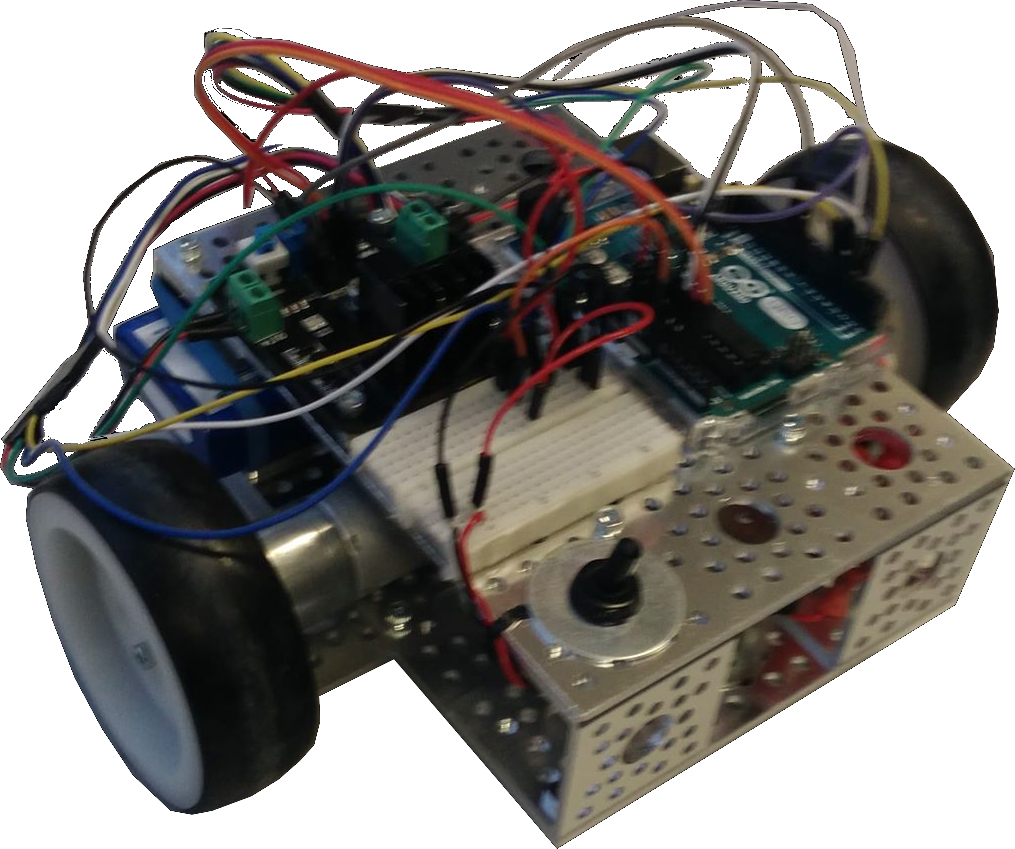
\includegraphics[scale=0.2]{base_roulante.jpg}
	\caption{Le prototype fonctionnel de base roulante}
\end{figure}

\section*{Acquisition de compétences et de savoirs}
\subsection*{Compétences et Savoirs}
\begin{itemize}
	\item Création de contenu de formation
	\item Formation des nouveaux membres
	\item Pédagogie
	\item S'exprimer devant un public
	\item Aprentissage en autodidacte (Surtout programmation)
	\item Transmission de l'information
	\item Création de codes clairs, concis et formatés
	\item Capacité de comprendre des codes existants
	\item Rigueur
\end{itemize}
\subsection*{Connaissances}
\begin{itemize}
	\item Utilisation avancée d'Arduino
	\item Conception et contrôle d'une base roulante en position
	\item Git et GitHub (Outils de versionage)
	\item Asservissement numérique
	\item \LaTeX
	\item Impression 3d
\end{itemize}
\subsection*{Projet réalisés et en cours}
\subsubsection*{Réalisation de formation Arduino}
\begin{itemize}
	\item Conception des formations, réalisation de codes à trous pour contrôler des systèmes de plus en plus compliquer (led, bouton, servomoteur, moteur à courant continu, liaison série, potentiomètre, capteur de distance ultrason…) : 5h
	\item Formation des nouveaux membres sur cette formation : 8h (deux séances le samedi)
	\item Correction et amélioration des formations grâce aux retours : 2h
\end{itemize}
\subsubsection*{Conception et contrôle d'une base roulante}
\begin{itemize}
	\item Recherche sur l'asservissement numérique d'un moteur avec encodeur à quadrature de phase : 5h
	\item Recherche sur l'asservissement de deux moteurs pour la base roulante : 5h
	\item Recherche sur l'asservissement de deux moteurs pour la base roulante : 5h
	\item Implantation basique de ces méthodes et test : 10h
	\item Recherche de solutions techniques utilisé par les autres équipes, lecture de leurs documentations et compréhension de leurs codes de contrôle : 5h
	\item Implantation des nouvelles fonctionalitées, débogage, tests, réglage, ceci répété plusieurs fois : 20h (toujours en cours)
	\item Formation des membres de l'ARTS sur ce projet : 4h
\end{itemize}

J'ai d'ailleurs utilisé tout le long de mon projet Git, un gestionnaire de version qui permet de revenir en arrière en cas de problèmes. Je l'ai utiliser avec GitHub qui permet d'avoir une version en ligne et pouvoir partager le code.
De plus, j'ai fait des formations sur ce projet pour transmettre ce que j'ai appris.

\subsection*{Projet}
\subsubsection*{ROS}
Apprentissage de l'utilisation de ROS, c'est un ensemble d'outils informatiques open source permettant développer des logiciels pour la robotique (cf.Wikipédia). Cela sera utile pour la gestion de robot complexe, comme le bras robotique actuellement développer par un projet ingénieur.

L'apprentissage de l'utilisation de ROS pourra être évalué par un document résumant sont utilisation et les codes commentés réalisés.

Temps estimé : 20h

\subsubsection*{Dynamixel}
Apprentissage de l'utilisation de Dynamixel, ce sont des actionneurs (moteurs) très performants, très utilisés dans la robotique.

De même que pour ROS, un document résumant son utilisation sera créé.

Temps estimé : 10h

\subsubsection*{Formation Arduino}
Compléter la formation Arduino avec des fonctionnalités avancées (interruption, timer…), et ajouter les corrections des formations.

Temps estimé : 5h

\subsubsection*{Encadrement des différents équipes (Mécanique, électronique, programmation)}
Pour la Coupe de France de Robotique, il est nécessaire d'avoir un planning pour les différents parties des robots, superviser l'avancée et encadrer les équipes.

Temps estimé : 1-2h/semaine

\subsubsection*{Programmation du robot}
La base roulante actuelle n'est qu'un prototype. Elle est donc vouée à changer, il faudra ainsi adapter le code en fonctions. Pour faciliter ce changement il est prévu de modifier le code tel que les différentes fonction du robot sont indépendantes (contrôle des moteurs, odométrie, génération de trajectoire…).

De plus il faudra implanter une stratégie de déplacements et d'actions.

Temps estimé : 3h/semaine

\end{document}